\documentclass[12pt]{article}
\linespread{1.3}
\usepackage{amsmath}
\usepackage[inner=2cm,outer=1cm]{geometry}
\usepackage{graphicx}
\title{Master Project - Draft }
\author{Duong Than}
\date{\today}
\begin{document}
\maketitle	
	
		\section{Introduction :} 
		\subsection{Background} 

			Public health officials are interested in finding hot spots where disease's risks are unusually high. They want to have an immediate attention to any disease clusters and also potential disease hot spots in order to implement prevention programs before it is too late. \\ 		
In such demand, researchers have been studied on different methods to detect disease clusters, and there are many of ideas that approach the use of point and regional count data to come up with an optimized solution. \\
			\textbf{What is a cluster?} A disease cluster defined as a zone of some connected regions that has an unusually high value of proportion between observed cases and expected cases, t-value, while the probability of anywhere else in the study area has a higher value than t is relatively small. \\
			
			\textbf{An example of an appearance of disease clusters:} There is a state in America where some disease is seen to have abnormal observed cases in some counties in this state. Public Health officials worry about the uncontrolled spreading of this disease, so they want to know exactly where the observed cases are significant high and where could be the next hot spots. The data of observed cases and population of each region can be assessed. So our ideal solution is to find some zones (could be more than one connected regions) where the observed cases are statistically significant high, and the rest of zones are not statistically significant high. It means if we can find all the connected zones and calculate those statistic tests, we will find the true disease clusters. However, if the number of regions are large, it is not feasible for us to be able to find all the connected regions within the study area. This problem comes down to why we need to come up with clever ways to find some "reasonable " subsets of regions in where it is feasible for us to find all the connected regions (zones). Further more, with respect to statistics, there are some restrictions for our zones. Since we do not want to consider a zone with many regions and with a very large population, so each zone has a limit of number of regions and the total population of each zone has to be less than or equal a half of the entire study area's population. These restrictions help us to reduce the size of possible zones of the entire study area. However; datasets can be varying in many ways, we still need to come up with more leverage methods of finding appropriate zones to detect for clusters. \\       
			
			\textbf{Objectives:} One of the main purposes of this paper is to compare and contrast these three existing methods. Also we want to approach this problem from a graph theory's point of view. In addition to those, we will propose some improvements based off of these methods. But first, we want to introduce how a dataset is formed in this problem. \\
				
		\subsection{Data Structure:} 
			In this section, we go into more detail about the data typically observed, standard assumptions about the dataset. 
			The basic form of the data involves a set of \textit{counts observed} (one count for each region ) and a matching set of \textit{counts expected} reporting the number of cases we expect in each region, under the null hypothesis which is everyone in the entire study area has the same constant risk. \\
			
We often assume that the data represent a set of counts arising from a \textbf{Heterogeneous Poisson process}.
In particular, many methods model the regional counts as independent Poisson random variables based on one of the basic properties of a spatial Poisson process : events counts from non overlapping regions follow independent Poisson distributions where the underlying intensity function defines the expected values ( and variances). Also, spatial data is non negative and discrete which are the two main properties of Poisson distribution. \\
			 
			
			
			As an example for the structure of a spatial dataset, we have an access to the Leukemia dataset for 218 regions in New York. This dataset contains 218 observations related to leukemia cases in 8 county areas of the state of New York. The data were made available in Waller and Gotway (2005) and details are provided there. In this paper, we study about geographical regions and their connected neighbors. And 			
the below graphics is an illustration of a study area and regions in it. For example,we want to look at a center region 83, and we want to study its five nearest neighbors. The algorithm to determine the nearest neighbors is to use the Euclidean distance to find the five centroids that have closest distances to centroid 83. Thus the five nearest regions of region 83 which are 89,90,84,88, and 75, and following figures are an illustration for a region and its nearest neighbors. \\	
			
		\begin{tabular}{|c|c|c|}
			
		\hline
			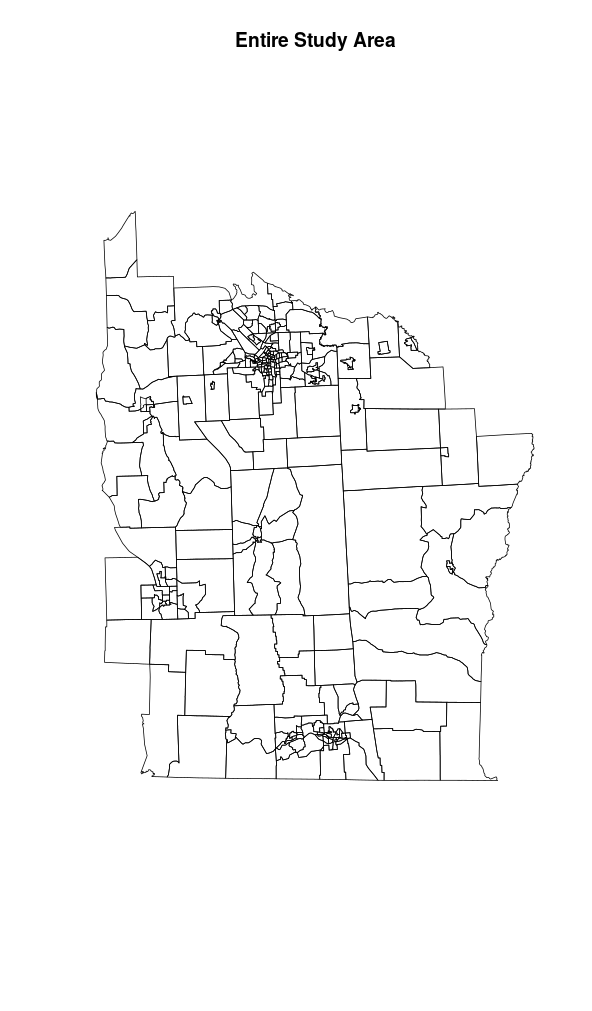
\includegraphics[scale=0.2]{nyplot.png}
			  & 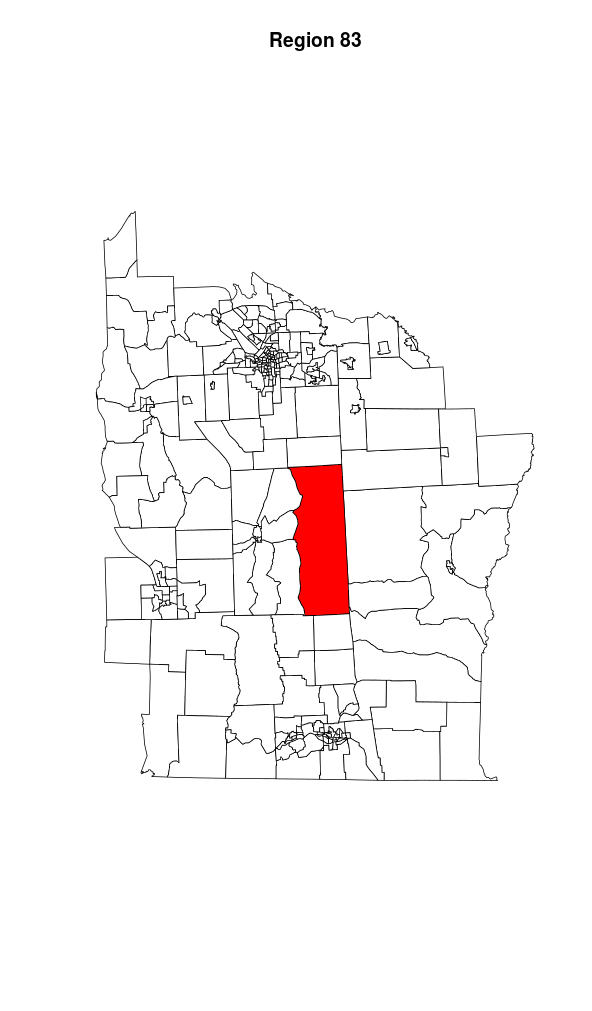
\includegraphics[scale=0.2]{ny83.png}
					&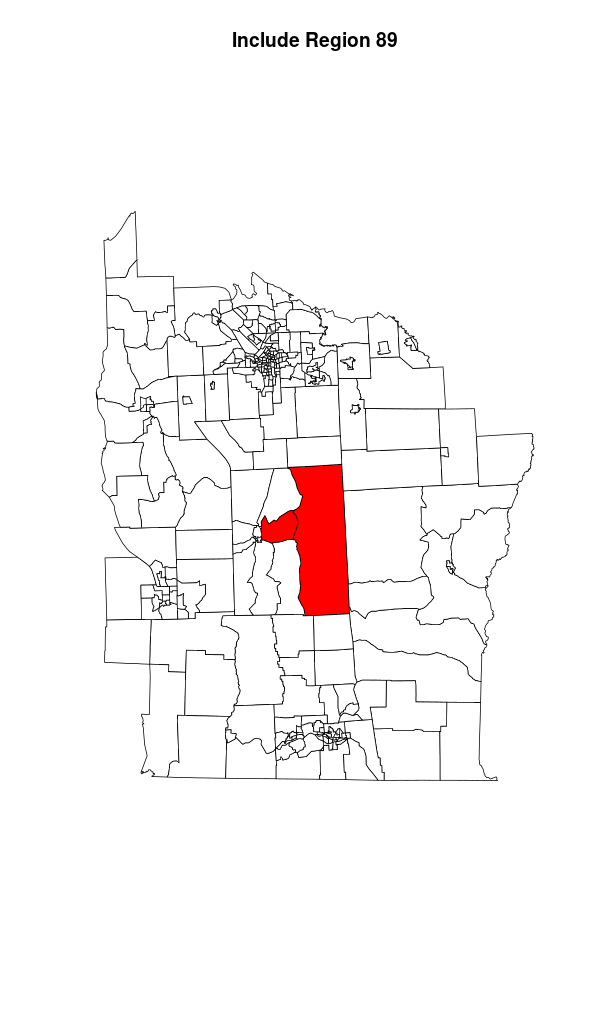
\includegraphics[scale=0.2]{ny89.png} \\ \hline
						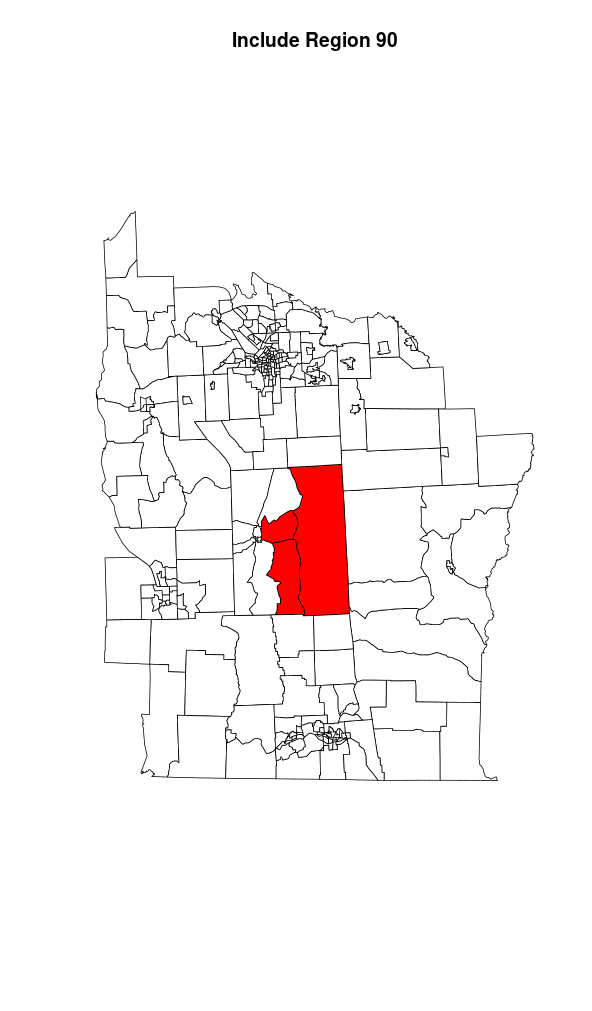
\includegraphics[scale=0.2]{ny90.png}
							& 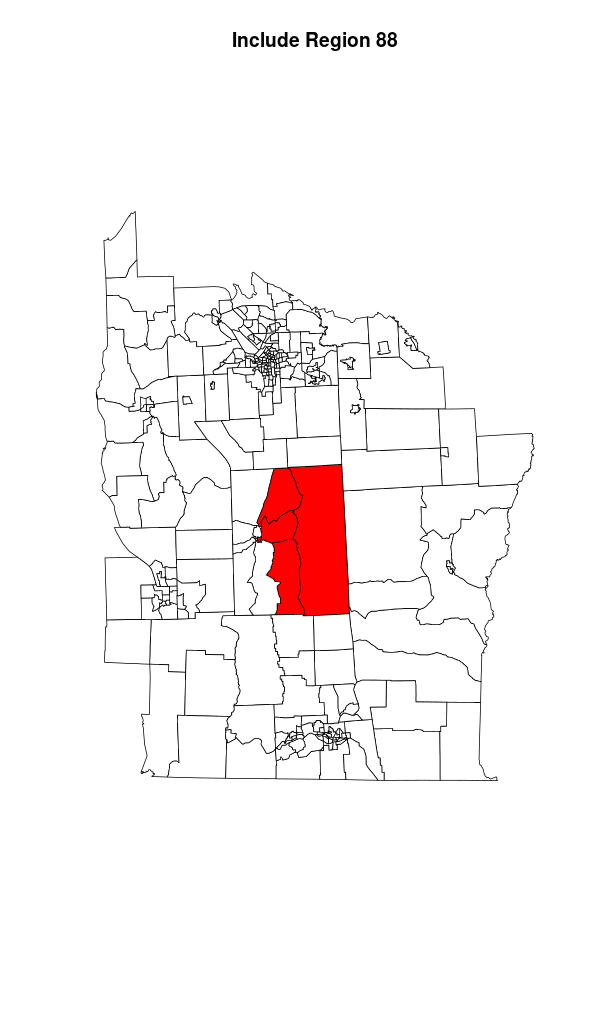
\includegraphics[scale=0.2]{ny88.png}
							   & 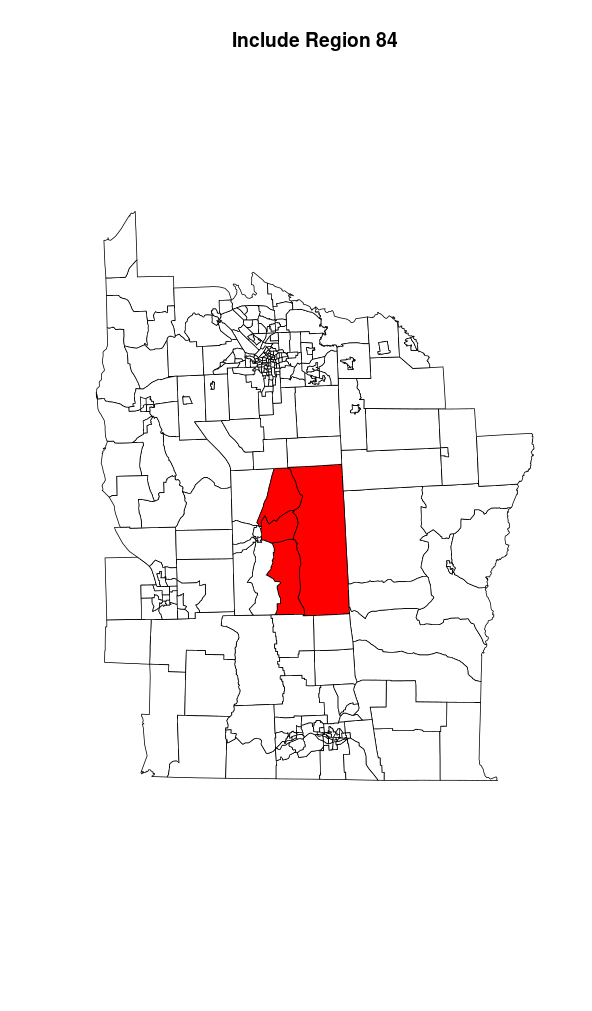
\includegraphics[scale=0.2]{ny84.png} \\ \hline
									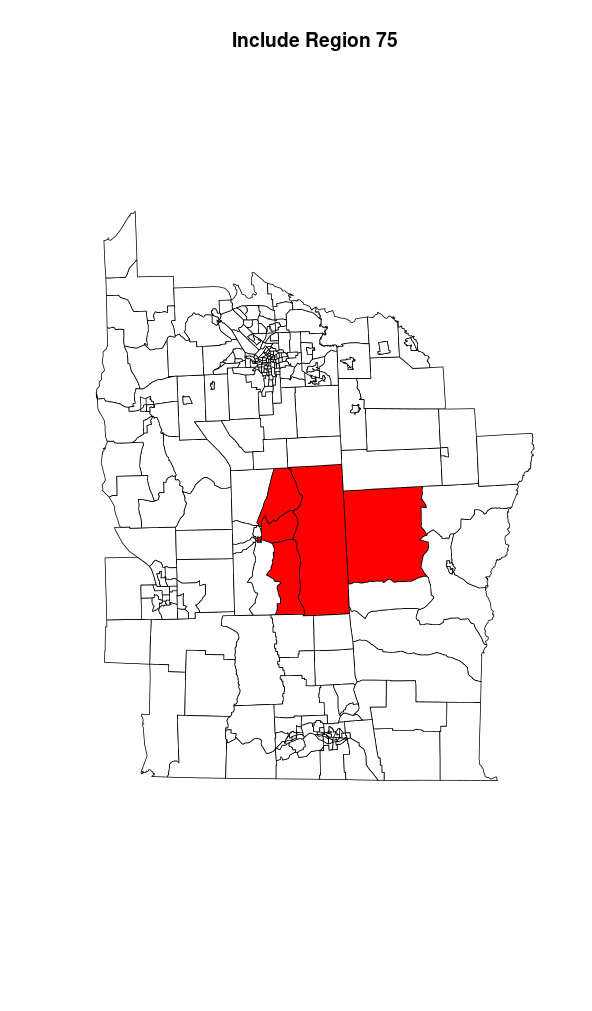
\includegraphics[scale=0.2]{ny75.png} && \\
		\hline	
			%\includegraphics[scale=0.2]{centroid.png}	\\
		\end{tabular}	\\
			The data $Y_1,Y_2,\dots,Y_N$ in regions $1,2,\dots,N$ are mutually independent Poisson random variables, where $Y_i$ are the observed cases in region $i$. \\ 
			And the associated population of each region is $n_1,n_2,\dots,n_N$. In this problem, we want to use the counts observed in each region to determined where the risk is unusually high.\\
Table below is an example of a dataset, which include region 83 and its five nearest neighbors, was extracted from the Leukemia New York dataset: \\

		\begin{tabular}{|c|c|c|c|}
		\hline
		Region & Population $(n_i$)& Observed Cases $(Y_i)$ & \\ 
		83 & 5532& 3.33995 & \\
		89 & 2921& 8.1795 & \\
		90 & 3711& 5.22804 & \\
		84 & 2592& 1.15928 & \\
		88 & 3242& 2.19922 & \\
		75 & 4189& 0.50936 & \\
		\hline
		\end{tabular}\\
			
			\subsection{Method:} 

			For the most part, methods to assess clusters and clustering in count data assume some background information on the entire population rather than a set of controls. 
			We divide the entire study area into N regions $ i = \{1,2,\dots,N\}$. \\
			Since we consider the population sizes $n_1,n_2,\dots,n_N$ fixed ,the total population in the study area is : \\
\[
n_+ = \sum_{i =1}^{N}n_i
\]
is also fixed. \\
Let $Y_+ = \sum_{i=1}^{N} Y_i$. If we condition on $n_+$, the total number of observed cases, we get the probability $ r = \dfrac{Y_+}{n_+}$, which is a fixed constant risk for all the individuals.\\
		
			\textbf{Test Hypothesis :} \\ 
			Let $Z$ be a collection of connected regions which we call zone $Z$. \\
			We define $Y_+(Z) = \sum_{j \in Z} Y_i$ , and $E(Z) = r*\sum_{i \in Z} n_i$. \\
			
			\textit{Null hypothesis :} Observed cases of each region equals to its expected number of cases. \\ 
			\begin{center}
			$H_0 : Y_i = E_i$ for all $i$
			 \end{center}
			 where $E_i$ are the null expected number of cases in region i. Also, $E_i = r * n_i$.\\
			
			
			\textit{Alternative hypothesis :} There is at least one zone for which the underlying risk is higher when compared to the null hypothesis. \\
 			\begin{center}
			$H_1$ : $Y_+(Z) \geq E(Z)$. \\
			\end{center}	
			With the assumption of Poission Process, below is the test statistic of likelihood ratio test for spatial clustering developed by Kulldorff : \\
				\[
					T = max_{z\in Z} \bigg[\dfrac{Y_+(Z)}{E(Z)}\bigg]^{Y(Z)} \bigg[\dfrac{Y_+(Z^c)}{E(Z^c)}\bigg]^{Y_+(Z^c)} I\bigg[\dfrac{Y_+(Z)}{E(Z)} > \dfrac{Y_+(Z^c)}{E(Z^c)}\bigg]
				\]	  (1)
		
				where $ Z^c$ denotes all the regions outside zone Z, and Y() denotes the observed cases within a zone, $E()$is the expected number of cases within a zone and I() is the indicator function. \\ 
			
			 \textit{Commentary}: A zone is considered as a cluster when its T-value is high enough so that it has to be statistically significant at the 0.05 level. Note that different techniques of picking potential clusters resulted in different T-value thresholds which determine whether clusters are statistically significant. \\
			 
			 \textbf{To determine significance:} \\
			 \begin{enumerate}
			 \item Calculate the test statistic of the observed data.	
			 \item Re-calculate it using a specified number (eg, 99, 499, etc.) of simulated data sets or permuation. This calculation is used to generate the expected distribution of the test statistic under the null hypothesis. 
			 \end{enumerate}
			 If A zone whose T-value falls into the $5\%$ of the extreme values of the expected distribution of the test statistic, it is statistically significant. \\
			
			\textbf{Restrictions for a target zone : } As we mentioned earlier, philosophically there are some restrictions for clusters. For each region's centroid , we determine $k$ (nearest) neighbors such that : \\
				\begin{enumerate}
					\item The farthest nearest neighbors from the centroid is less than or equal the max distance $d$ which depends on the dataset. \\ 
					\item The population of zone is less than or equal a half of the entire study area's population. ($n(Z) \leq 0.5(n+)$).\\
				\end{enumerate}
			
				\subsection{The Problem Under Graph Theory's Point of View} 
				
				Since we are working with spatial data, it is interesting to translate this problem into a graph theory problem from which we can use some graph theory's techniques to find clusters. 
				%A centroid of each region is picked at the location where it has the biggest density of population of the region. 
				
				Firstly,we want to introduce the problem in graph theory's terminology. We let the entire study area be a graph $G$ where : \\
				\begin{enumerate}
					
				\item $V(G)$ is the set of all the centroids. Each vertex of $G$ is a centroid. \\
				\item $E(G)$ is the set of all the two centroids which represent for a pair of regions that share their boarders together. Each edge of $G$ represents for a pair of regions that share boarder together.\\
				\end{enumerate}
				
				Each vertex of $G$ contains information of each region that it represents. For instance  each vertex contains observed cases, expected number of cases and population.
				
				A clusters is some induced connected subgraph $G[H]$ that could give us the maximum value of the statistic test (1). Regardless to which method is used, a cluster is an induced connected subgraph of $G$ and has at least following properties : \\
				\begin{enumerate}
					
					\item $|H| \leq k $ where $H$ is the set of vertices of this induced connected subgraph.
					%\item $ \forall v_i \in  V(G[H]), d(v,v_i) \leq d $
					\item $n(H) \leq 0.5(n_+)$ where $n(H)$ is the total population of vertices/regions $v_i \in H$. 
				\end{enumerate}
				Also depend on different methods, there maybe be more properties for induced connected subgraphs that are considered as clusters.\\ 	
			
				Combinatorially, there are total $2^ {\binom{N}{2}}$ induced connected subgraphs in $G$. When $N$ is large, it is almost impossible for us to search for clusters within this many number of possible zones. In theory, we are able to find all the induced connected subgraphs of a given graph in order to find true clusters. However, when the graph is large enough, it is not feasible to do so. Thus, the question is: how to find a clever way to search a large enough to make the search computationally feasible but not all number of induced connected subgraphs that would include all the true clusters? That is the reason why researchers have been proposing different methods for this question. The next section will introduce us to the three main existing methods on finding clusters in a reasonable running time of searching.\\
			
			
\section{Existing Methods :} 
			
				There are three different spatial scanning methods has been proposed : Circular Scanning Test, Upper Level Set, and Flexible Scanning Test. Those use similar likelihood ratio test to determine which regions could be potential disease clusters using a particular spatial data. However, those approach different ways of forming sets of zones to be tested.\\			
				\begin{enumerate}
			\item \textbf{Circular Scanning Test} : Kulldorff detected potential clusters (zones) for the study ares by making circles $(C_i)$ whose the center is the centroid of each region $i$, and determine the radius of each circle by using the following steps : \\
	
			\begin{enumerate}
				\item Starting at a centroid $i$. 
				\item Applying a relative small radius of $C_i$ to begin the scanning window. Each scanning window contains a center $i$ of region i ( the centroid of a region i ) with all the regions whose centroids fall into the current circle. 
				\item Increasing the length of radius of $C_i$ until either the radius meets the max distance or the scanning window contains $k$ regions or the current zone's population exceeds $0.5(n+)$. A new formed zone $(Z_i)$ has the center is the centroid of region $i$ and includes all the regions whose centroid falls into the current circle. 
				\item Applying those steps to every single region of the entire study area to find all the possible candidate zones. 
			\end{enumerate}  
		In this method, at each region, we conduct a search around it, and the scanning window can contain a maximum of k regions in it. Thus the total number of possible candidate zones is N*k which is feasible to conduct a search.
		As the result, the zones with highest T-value and is statistically significant within each scanning window were decided to be clusters. \\
			
			There are some advantages of this method. We search for potential clusters using every single regions. We can find all the potential zones in a linear time. For each region we start the search, there are maximum k zones as the results. Thus, there are maximum $n(k)$ running times. However, there are some disadvantages we encounter. We define a hole is a region that has no observed cases. Firstly, there would be holes in zones. Since we determine our potential zones using geographical distance, some holes might be included in some zones which will not help to increase the t-value of those zones. Secondly, the shapes of the zones are most likely to be circles whereas geographical zones can be in more complicated shapes. Thirdly, since we keep increasing the radius of the zone until it meets one of the restrictions, we might neglect a single region as a potential zone itself. \\  
		In graph theory's point of view, to find all the potential zones, we start a a vertex. From a vertex $v$, we find an induced connected subgraph $G[H]$ with the following properties : \\
				\begin{enumerate}
					
					\item $|H| \leq k $ 
					\item $ \forall v_i \in  H, d(v,v_i) \leq d $
					\item $n(H) \leq 0.5(n_+)$ where $n(H)$ is the total population in centroids $v_i$. 
				\end{enumerate}   
				Remark (not sure if this is how they run the test) : For each time we increase the distance from $v$ and there is a new centroid drop in, we calculate the T-test. Then for each center region, we can find the connected zone which has the highest T-value. \\ 
				
	
	The figure below is an demonstration of the scanning process of the Circular Method where region 11 is the original region of the search:\\
	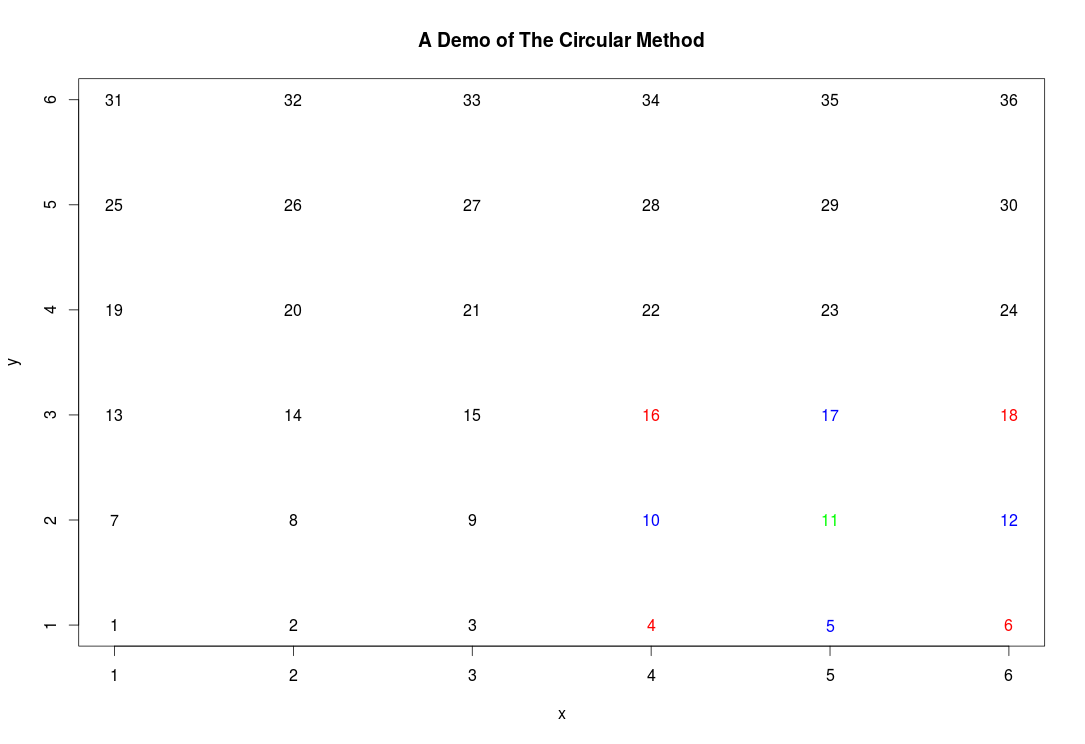
\includegraphics[scale=0.45]{demo_1} \\
	For the radius of 1, regions 10,12,5,17 are the nearest neighbors of region 11.\\
	Then we increased the radius up to 1.5, regions 4,6,16,18 are the nearest neighbors of region 1.\\
	In this example,three candidate zones that are formed: \\
	\begin{enumerate}

	
	\item Candidate zone 1: region 11\\
	\item Candidate zone 2: Regions 11,5,10,12,17\\
	\item Candidate zone 3: Regions 11,5,10,12,17,4,6,16,18\\
	
	\end{enumerate}
	 
	 \item  \textbf {Upper Level Set (ULS) Scan Statistic :} \\
			The ULS scan statistic is an adaptive approach in which the parameter space is reduced by using the empirical cell rates
\[
			 G_i = \dfrac{Y_i}{n_i}
\]
			They define the Upper Level Set is the set that comprises all the regions with each level $g$.\\
			\[
U_g = \{ i : G_i > g\}
			\]
 Within the each Upper Level Set, they form their target zones as the following: %		process : \\ 
				
				Let $ULS= \{1,2,\dots,t\}$ be the Upper Level Set of regions $i$ such that $G(i) \leq G(j)$ if and only if $i < j$.  
				\begin{enumerate}
					\item Region $1$ is the first zone $Z_1$. 
					\item If region $2$ connects to region $1$, then $2 \in Z_1$. If region $2$ does not connect with region $1$, then $2$ is $Z_2$. 
					\item Keep repeating this process until we run out of regions in ULS. \\   
				\end{enumerate}
			 In this method, the searching is reduced down to only $t$ numbers of regions instead of $N$.The total number of possible zones is less than or equal $t$ which is feasible to conduct a search. And a cluster is a zone within $U_g$ that has the highest T-value and is statistically significant compare to other zones within set $U_g$.\\ 
		An advantage of this method is the running times while searching is much smaller. There are maximum $t(k)$ times and $t \leq N$. \\	
		However, there is a disadvantage that we do not take consideration of all regions. Some regions with small $G_i$ values that give large $T-values$. \\
		
		If we look at this method under graph theory's point of view , a ULS set is a simple planar graph $H$. And our potential zones are the components $\{C_i\}_{i=1}^{t}$ of $H$. Also, each component $C_i$ has the same properties as each induced connected subgraph $G[H]$ in the circular scanning test. \\  
				
	
	The figure below is a demonstration of the scanning process of the ULS method. We set $g$ equals the mean of the observed cases of the entire study area.\\
	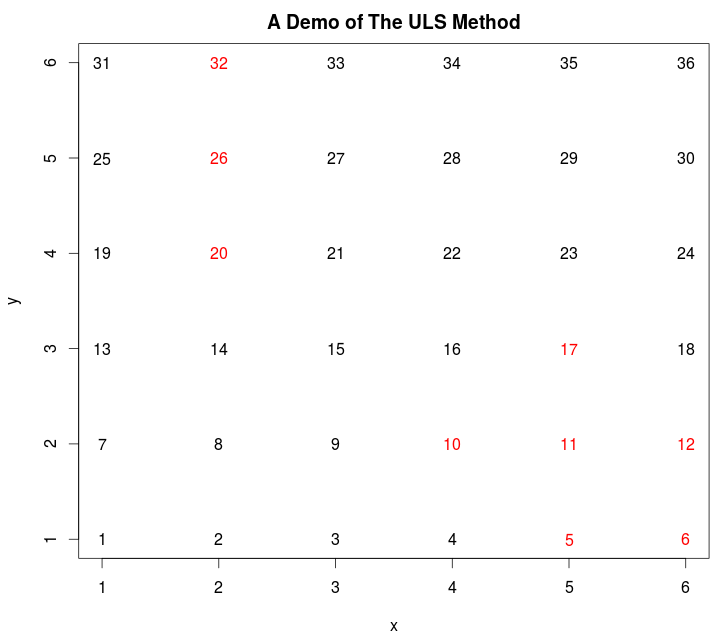
\includegraphics[scale=0.5]{demo_2} \\
	Red regions are regions whose $G_i$ is greater than the mean of the observed cases. As we can see that there are two different candidate zones that we need to look at. Now the total number of regions that we want to search for clusters are only 9 regions instead of 36 regions. This step reduces a significant times of searching for clusters. 
		\item \textbf{ Flexible Scanning Test:}	\\
			
			The flexible scanning test is a different method to pick up potential zones for clusters. In this method,the scanning window of each region i comprises a maximum k regions which includes region i and k-1 nearest neighbors of region i. Within these k regions, a cluster is the zone whose included regions are a subset of the k regions that is connected and has the highest t-value compare to other zones of these k regions. Thus, the potential zones can have a different shape rather than a circle which the author of this method claimed that this method is better than the circular method. \\
			
				Let $Z_{ik}$ denotes the window composed by the nearest ${k-1}$ neighbors to the region i.Thus all the windows are scanned by the spatial scan statistic are included in the set : \\
		\[
			Z = \{Z_{ik} | 1 \leq i \leq N, 1 \leq k \leq K \}
		\] 
				In this method, there are maximum $ N\sum_{i=1}^{k} i $ number of regions that are searched, which makes the clustering searching more feasible. However, $ N\sum_{i=1}^{k} i $ is quite a small number of zones compare to possible $2^{\binom{n}{2}}$ zones we could have in this study area. This raises a concern whether this method is sufficient in searching for clusters or not. \\
			
			In graph theory's language, clusters in this method are induced connected subgraphs of $G$ which have less than or equal k number of vertices. \\
			 	
		% Under the scanning test, our null and alternative hypothesis are : \\
			
		%	$H_0 : E(N(Z)) = a(Z)$ for all Z .\\
			
		%	$H_1 : E(N(Z)) > a(Z)$, for some Z. (There is at least one window Z for which the underlying risk is higher inside the window when compared outside.)\\
		%		where $N()$ is the random number of cases, and $ a()$ is the null expected number of cases. \\
	
		%	Under the Poission assumption, the test statistic, which was constructed with the likelihood ratio test, is given by : \\
				
		%		\[
		%			sup_Z(\dfrac{n(Z)}{a(Z)})^{n(Z)} (\dfrac{n(Z^c)}{a(Z^c)})^{n(Z^c)} I(\dfrac{n(Z)}{a(Z)} > \dfrac{n(Z^c)}{a(Z^c)})
		%		\]	 
	
		%		where $ Z^c$ denotes all the regions outside window Z, and n() denotes the observed cases within the specified window, and I() is the indicator function. \\ 
	The figure below is a demonstration of the scanning process of the Flexible method. Again, the original region is 11, and we set the maximum number of regions for each zone is k=7.\\
	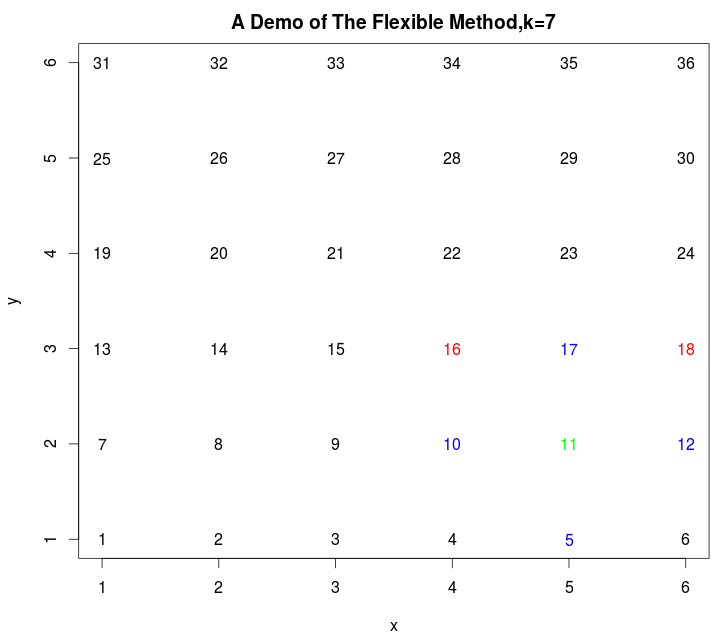
\includegraphics[scale=0.5]{demo_3} \\
	In this demonstration, we choose region 11 as the center region, then pick the first nearest region to 11 is 10,12,5,1. After all then first nearest regions are picked, the second nearest regions are picked and so on until we reach the maximum k. Thus,16 and 18,the second nearest regions to 11 are picked. Note that in this example, we can also pick 4 and 6 instead of 16 and 18. And this could increase the number of searching times. However, in real life, it is almost impossible for two regions to have the same distance to a third one. \\  
	
	In this example, we generated 14 candidate zones which are: \\
	
	
		
	
	\begin{tabular}{|c|c|}
		\hline
		Candidate zone & Regions  \\
		\hline
		1 & 11  \\
		2 & 11,5 \\
		3 & 11,10 \\
		4 & 11,12 \\
		5 & 11, 17 \\
		6 &  11,5,10 \\
		7 & 11,5,12 \\
		8 & 11,10,17 \\
		9 & 11,12,17 \\
		10 & 11,12,17,18 \\
		11 & 11,10,16,17 \\
		12 & 5,11,12,17,18 \\
		13 &  5,11,12,16,17 \\ 
		14 &   5,10,11,12,16,17,18 \\ 
	\hline
	\end{tabular}
	
	\section{A Contrast of the Three Methods Applied on the Leukemia New York Data}
	In this section, using the Leukemia New York data, we take a closer look at the differences among these three methods in determining their own clusters. \\
	The table below shows clusters of each method:\\
	
	\begin{tabular}{|c|c|c|c|}
	\hline
	& Circular & ULS & Flexible \\
	
	 & 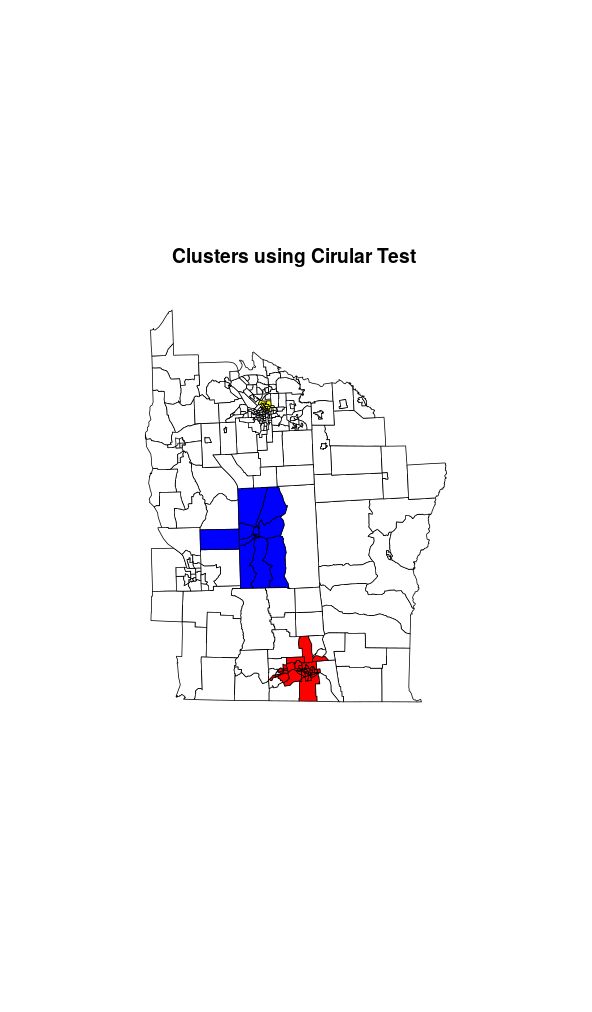
\includegraphics[scale=0.3]{cluster_circular} & 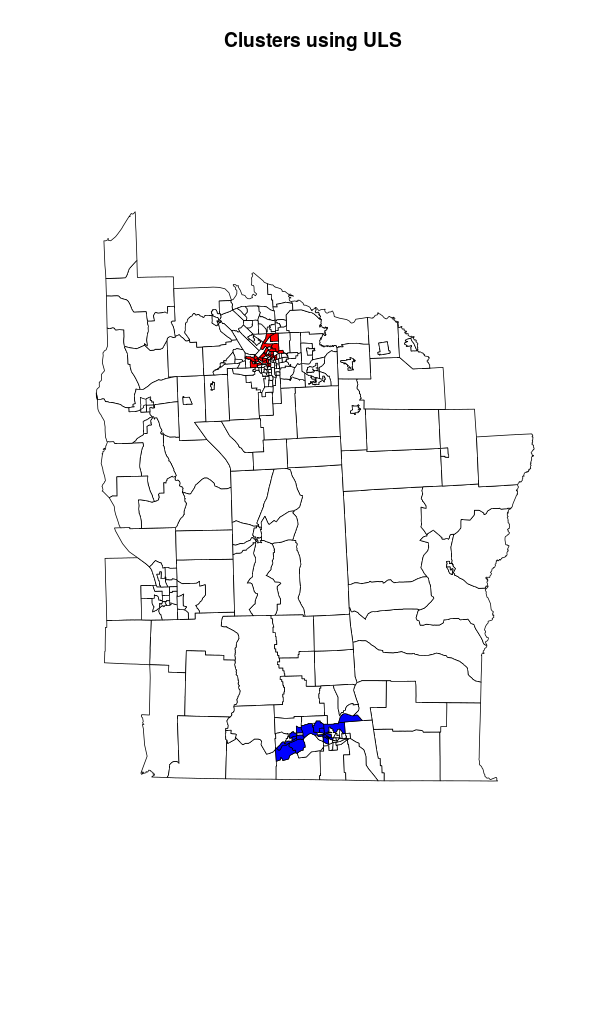
\includegraphics[scale=0.2]{cluster_uls} & 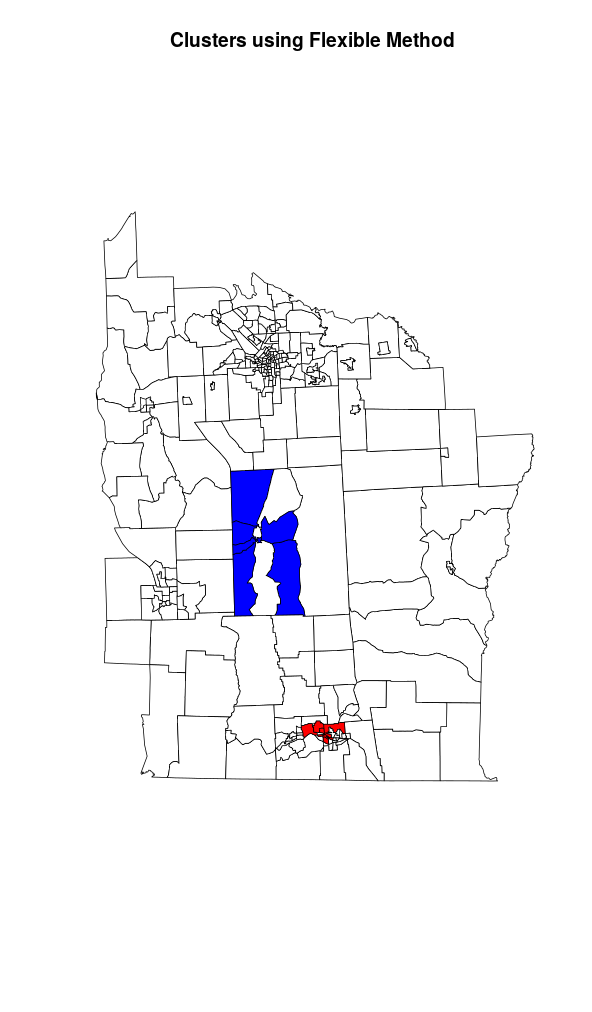
\includegraphics[scale=0.2]{cluster_flexible}\\
	\hline
	\end{tabular}
	
	 \subsection {Circular Method} 
	
	 \begin{tabular}{|c|c|c|c|c|}
	 \hline
	 & Observed Cases & Population & Log of T-value& P-value  \\
	Cluster 1: & 117 & 135295 & 15.00556 & 0.01\\ 
	Cluster 2:& 47 & 48501 & 7.851015 & 0.09\\
	Cluster 3:& 44 & 45667 & 7.199672 & 0.1\\
	\hline
	\end{tabular} \\
	
	\subsection{Upper Level Set Method} 
	
	 \begin{tabular}{|c|c|c|c|c|}
	 \hline
	 & Observed Cases & Population & T-value &P-value  \\
	Cluster 1: & 78 & 66679 & 21.61002 & 0.01\\ 
	Cluster 2:& 73 & 62749 & 19.86723 & 0.03\\
	% Cluster 3:& &  &  &\\
	\hline
	\end{tabular} \\
	
	\subsection{Flexible Method} 
	
	 \begin{tabular}{|c|c|c|c|c|}
	 \hline
	 & Observed Cases & Population & T-value & P-value  \\
	Cluster 1: & 39 & 31420 & 11.67128& 0.01\\ 
	Cluster 2:& 43 & 36446 & 11.64168 &\\
	 % Cluster 3:& &  &  &\\
	\hline
	\end{tabular} \\
	
	
	\textbf{Circular Scanning Method:} Three clusters have circle-like shapes, and each cluster includes more regions than the other two methods.\\
	\textbf{ULS Scanning Method:} The shape of the two clusters are different than circles. \\
	\textbf{Flexible Scanning Method:} The maximum number of regions for each cluster is restricted at 15.	
	The shapes of clusters in this method are more flexible than the circle shape in Circular Scan Method. These clusters are overlap with clusters in Circular method except it has only two instead of three clusters. \\
	
	\section{A Small Example}
	Although we have an access to the Leukemia dataset, it is easier to contrast the three methods using a smaller scale of dataset and the true clusters are known. This section will help us to see in a smaller example how each method pick up its clusters. So we created a dataset of a study area which had 36 regions. The spatial setup of this dataset is a $6\times6$ grid. The population for each region was randomly generated using Poisson distribution with the mean of 1 million. We picked in advance 2 true clusters. One cluster had 4 connected regions and the other one had 3 connected regions. The observed cases for each region was generated as the following: \\
		
	\begin{tabular}{|c|c|}
	\hline
	Regions & Observed Cases \\
	\hline
	7,11,12,17(Cluster 1) and 20,26,32(Cluster 2) & Observed cases = 0.005 * population \\ 
	4,5,10,14,15,18,24,23 & Observed cases = 0.002 * population \\
	1,2,3,6,8,9,13,19,21,22,25,26,28,29,30,31,33,34,35,36 & Observed cases = 0.001 * population \\
	\hline
	\end{tabular}	
	
	\end{enumerate} 
	
	This is the layout of our study area for our small examples:\\
		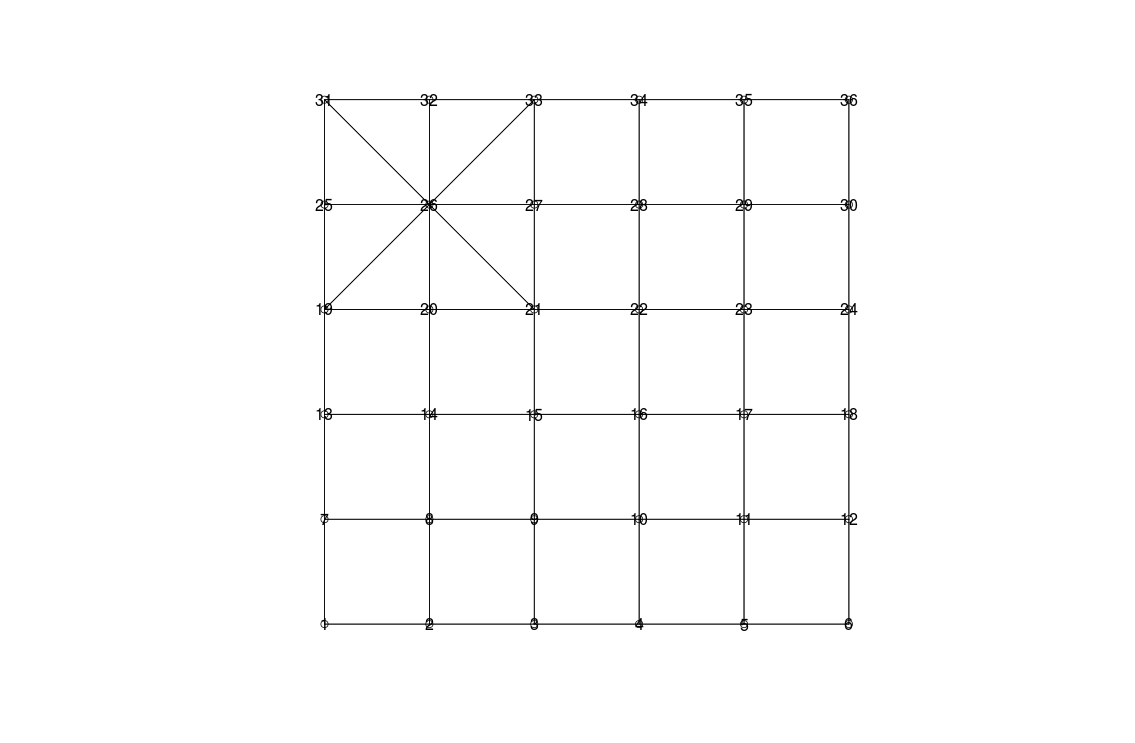
\includegraphics[scale=0.3]{Area_layout} \\
	
	And the figure below shows the density of the observed cases of each region in the entire study area.\\
	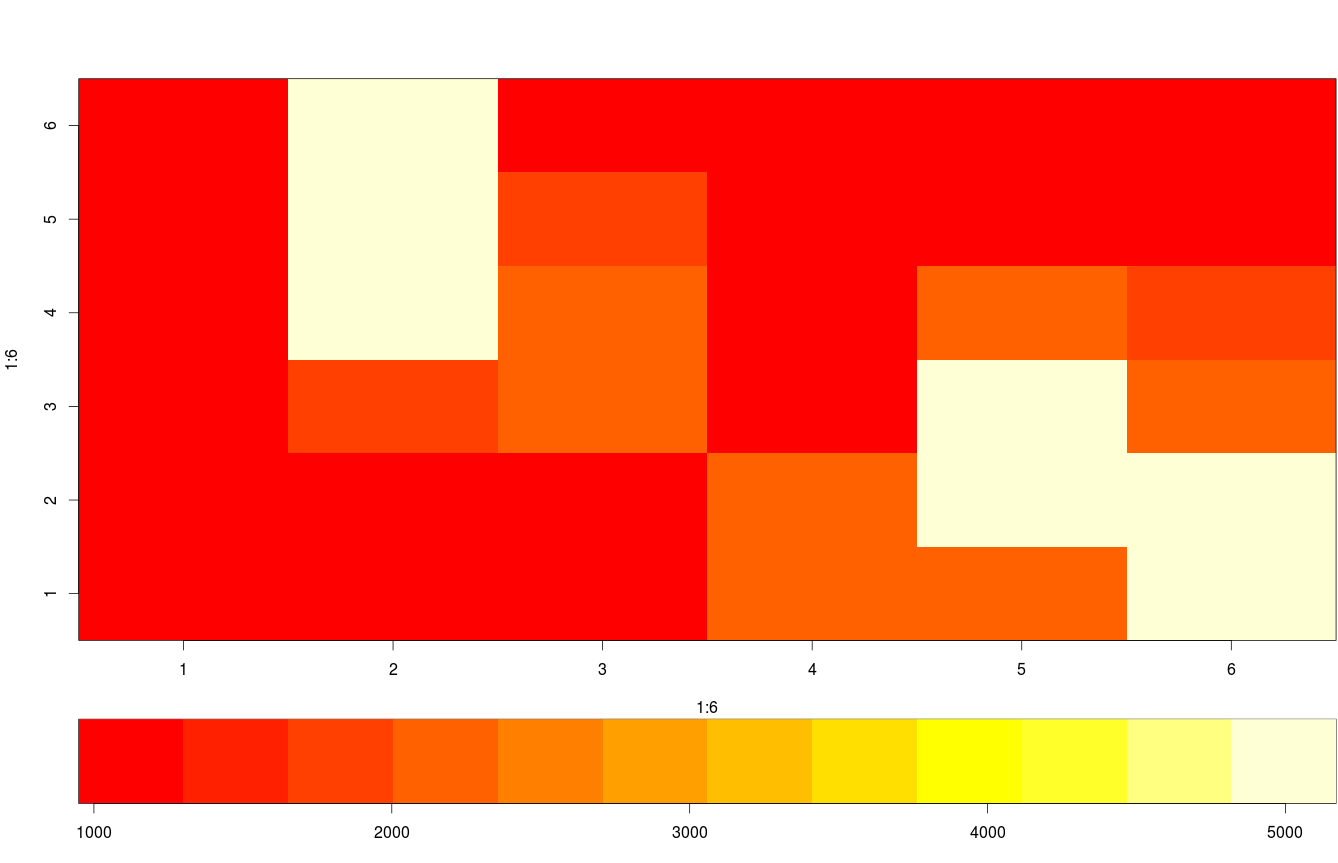
\includegraphics[scale=0.2]{density_cases}\\
	
	As we deliberately determined the two true clusters, the closest picture of our study area should have looked like the below graph: \\
	
	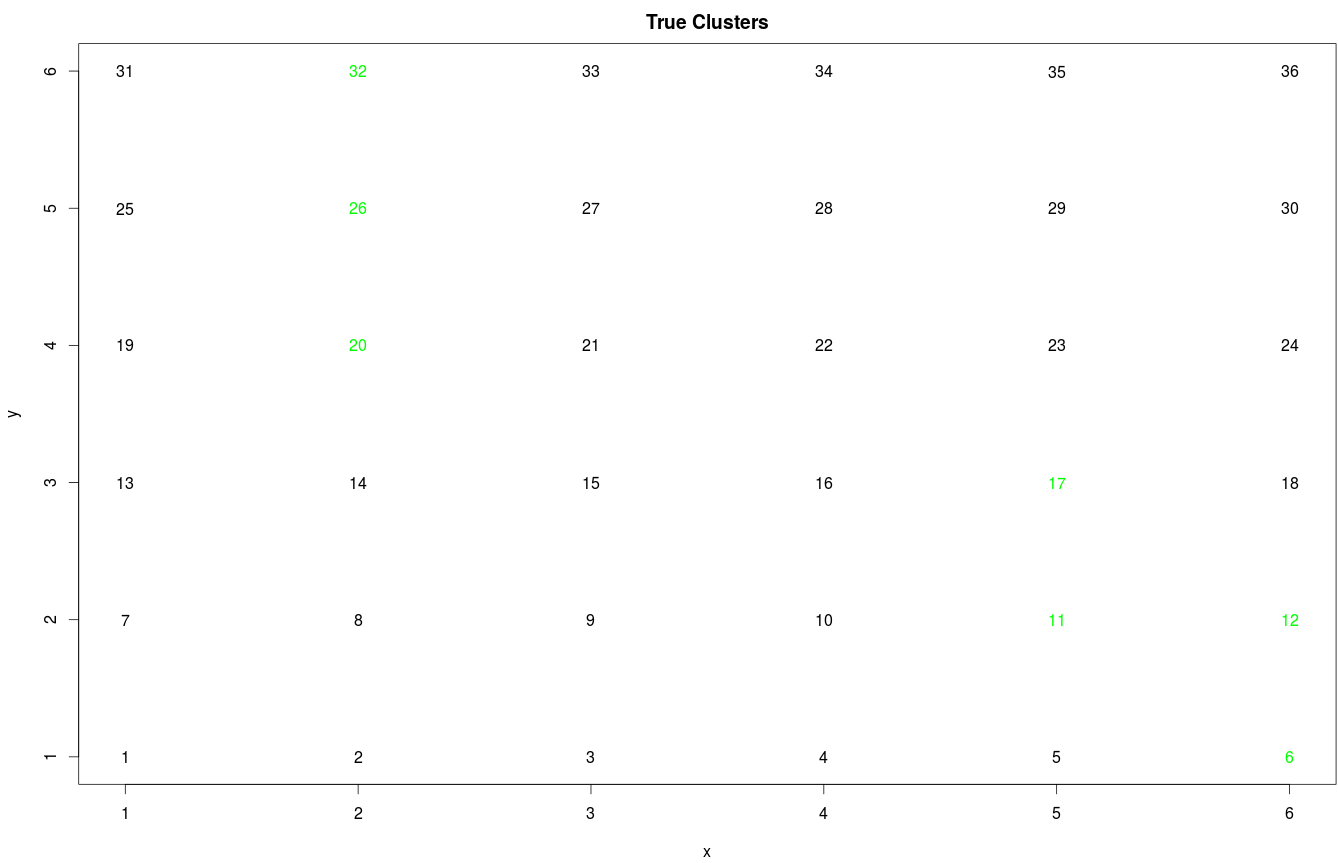
\includegraphics[scale=0.25]{true_clusters}\\ where the connected green nodes were divided into the two separating clusters. \\
	
	Then we tested the three methods using this dataset. \\
	
	\subsection{Clusters of Circular Test } 
	 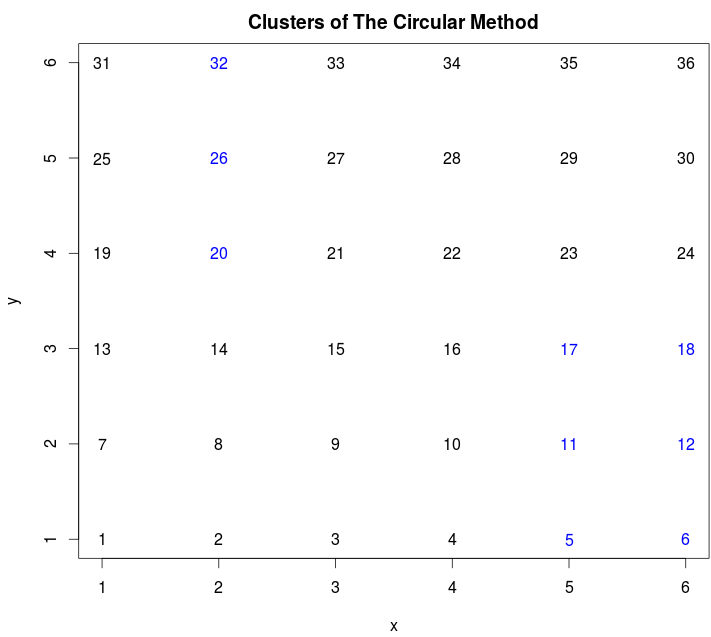
\includegraphics[scale=0.3]{test_1} \\ The circular method produced two clusters. One had 6 connected regions, and the other one had 3 connected regions. This method detected one true cluster. and it also detected the second true cluster but added two extra region in it. \\
	\subsection{Clusters of ULS Test}
	 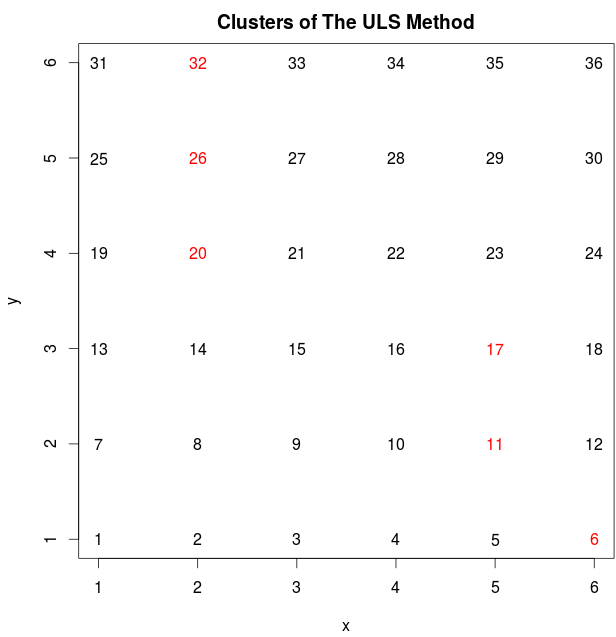
\includegraphics[scale=0.35]{test_2_01} \\ We found these two cluster using ubpop = 0.1. There were two different clusters as the result. Both clusters comprised three connected regions. But when using ubpop* = 0.2 the two clusters were slightly different which we can see in the below figure:\\
	 
	 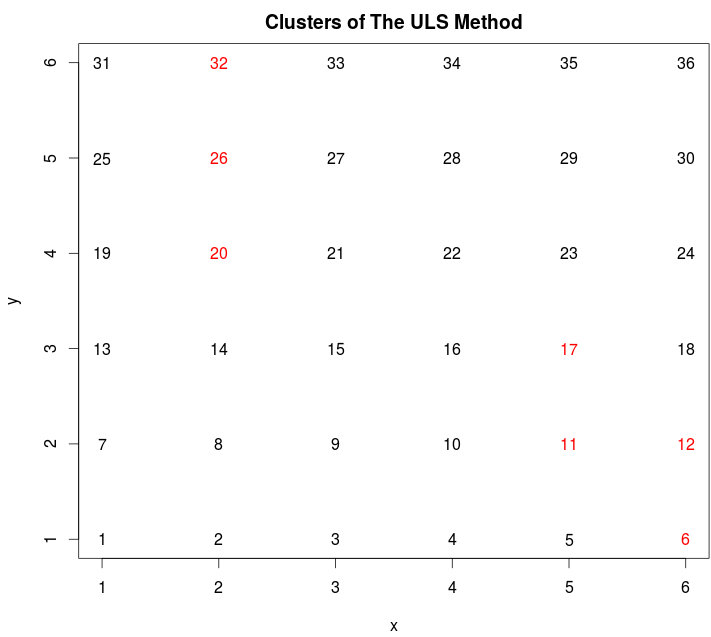
\includegraphics[scale=0.3]{test_2}\\ This result gave us exactly two clusters that we deliberately picked. Thus this method detected the right hot spots when we used an appropriate ubpop.  \\ 
	\textit{ubpop:} a proportion between 0 and 1 containing the upper bound for the proportion of total population contained collectively among a set of nearest neighbors.\\
	\subsection{Clusters of Flexible test} 
	 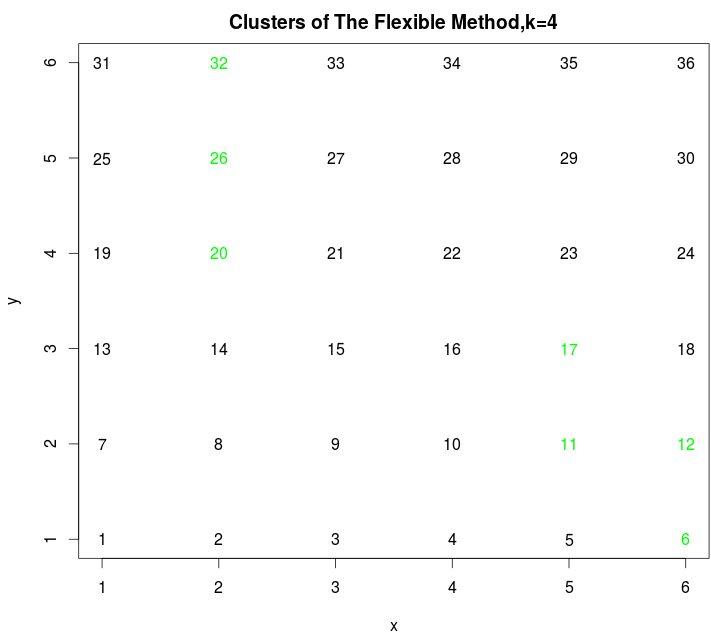
\includegraphics[scale=0.4]{test_3} \\ We found these two clusters when we ran this test with k=4 which were the true clusters.\\ 


\subsection{Conclusion}

In this small example,ULS and Flexible methods detected the true clusters with an appropriate setup of some parameters while the Circular method detected two extra regions to be considered as high risk spots. These results are compatible with the New York Leukemia data with respect to the size of clusters. In section 4, we found that the Circular method detected bigger size of clusters comparing to clusters of the other two methods. Thus we might suspect that the Circular method tends to detect more false hot spots than the ULS and Flexible methods. A possible explanation for this observation is in Circular method, candidate zones are in circle shape. Thus, a detected hotspot could include a few false regions if those are in the same zone with other true regions.  

To strengthen our suspicion, we tested another example with true clusters that had different shapes than our first example. We wanted to see if the results are consistent with our assumption about Circular method.\\ 
The following figure are shown the two true clusters.\\
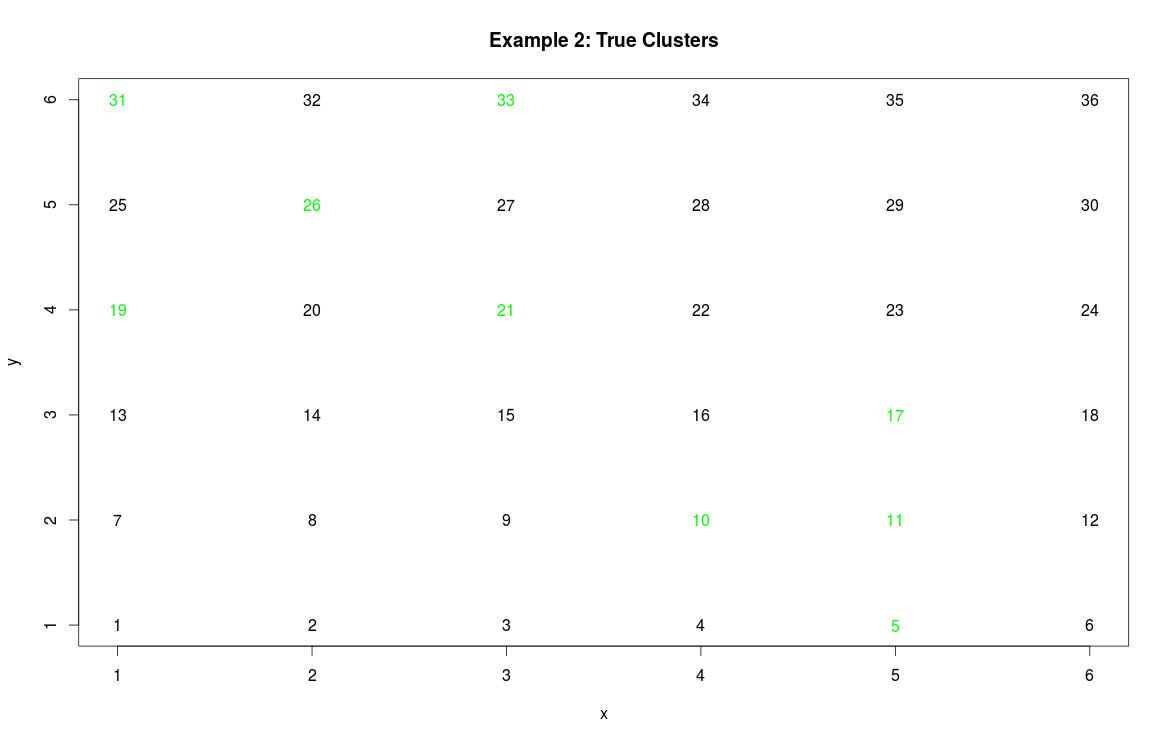
\includegraphics[scale=0.2]{ex2_true}\\

\hspace{4cm}\begin{tabular}{|c|c|}
	\hline
	Cluster & Regions \\
	\hline
	1 & 19,21,26,31,33 \\
	2 & 5,10,11,17 \\ \hline
\end{tabular} \\

First, we found 3 clusters using Circular method:\\
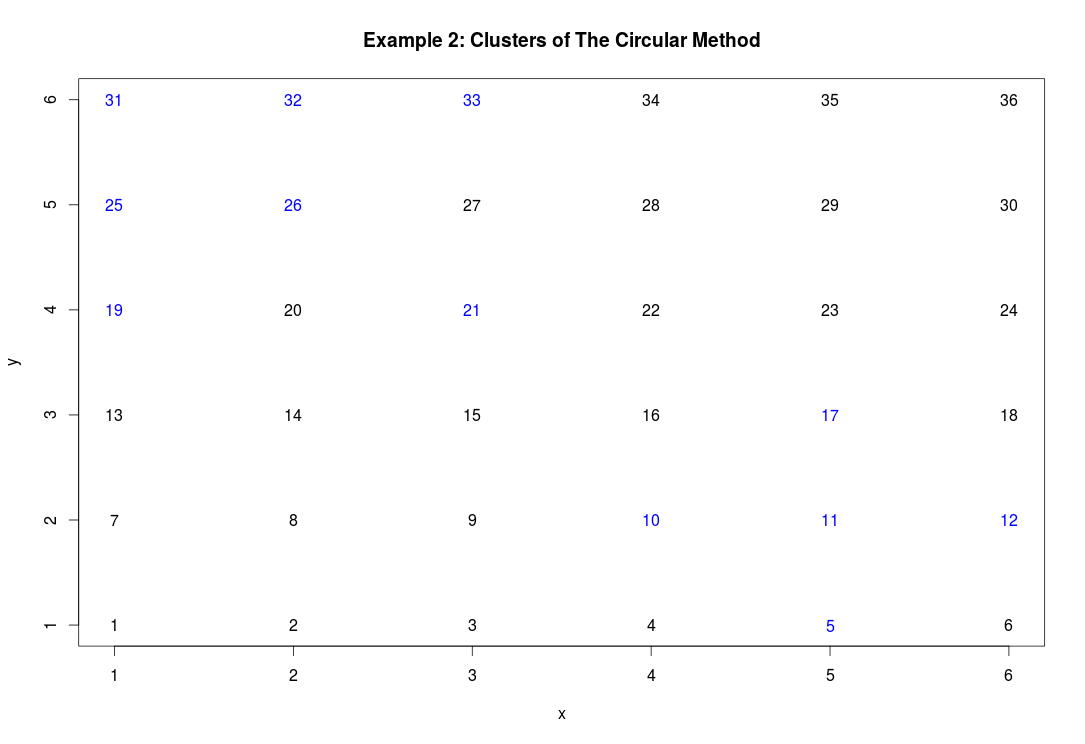
\includegraphics[scale=0.2]{Ex2:Circular} \\

\hspace{4cm}\begin{tabular}{|c|c|}
	\hline
	Cluster & Regions \\
	\hline
	1 & 19,25,26,31,32,33 \\
	2 & 5,10,11,12,17 \\ 
	3 & 21 \\ \hline
\end{tabular} \\

This results had not surprised us as clusters included three extra regions compare to our true clusters.\\

The next figure illustrates the clusters of ULS method: \\ 
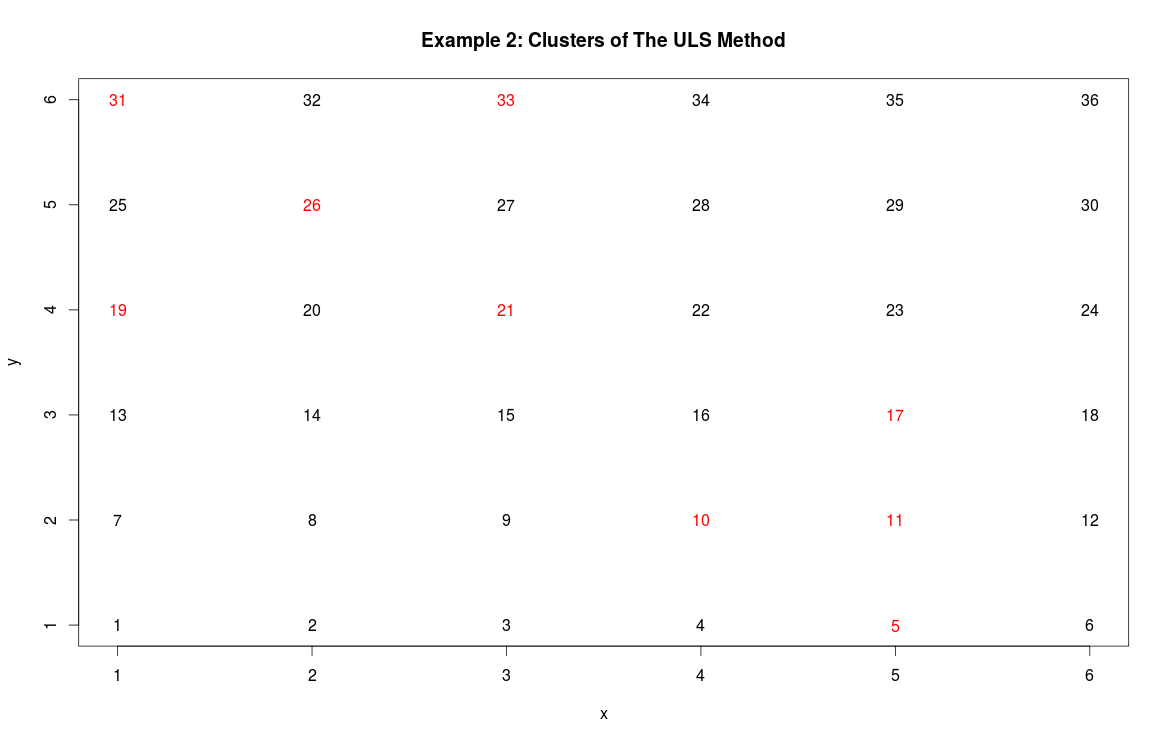
\includegraphics[scale=0.2]{Ex2:ULS}\\
With ubop = 0.3, the ULS method picked up the right true clusters.\\

And this is the results using Flexible method:\\
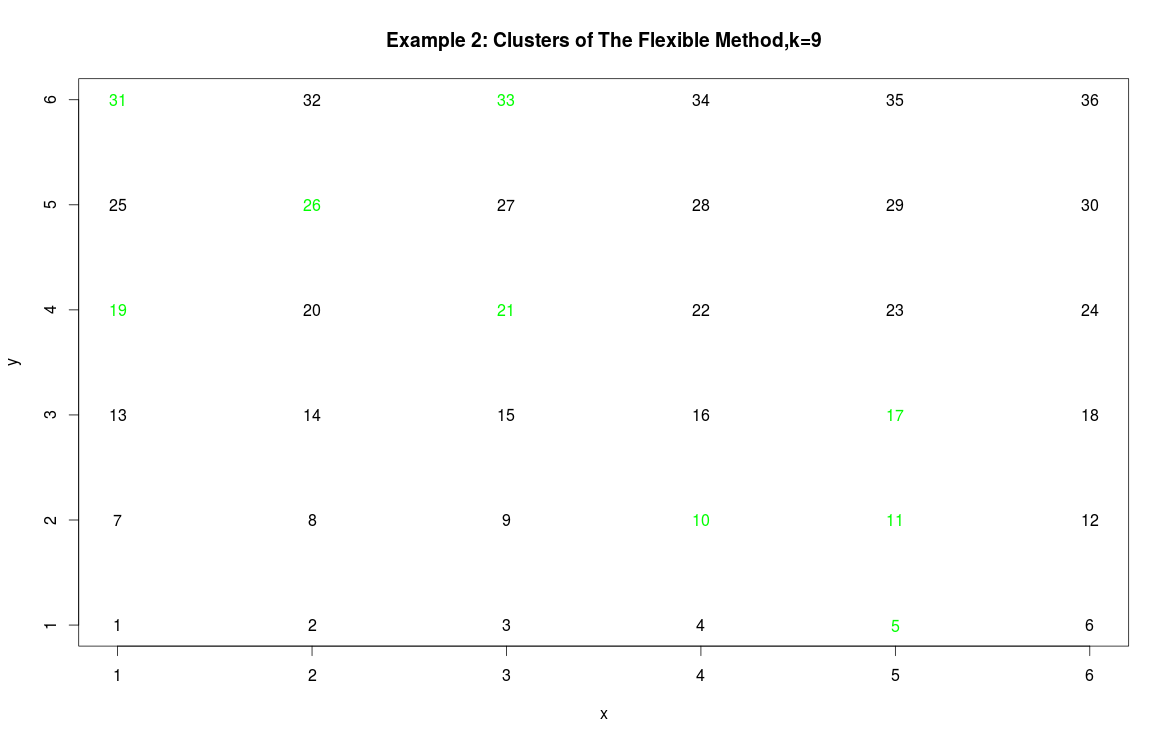
\includegraphics[scale=0.2]{ex2:Flexible}\\
In this example, in order for Flexible method to pick up the right true clusters, we need to increase $k$ value up to 9 which unexpected since the largest size of our true clusters was five. \\

So there are trade offs between using Circular and Flexible methods. The technique of selecting candidate zones of Circular method and Flexible method are similar since they tend to pick the nearest neighbors of a given center zone. However, using Flexible method, we have more candidates zones, and we can find the true clusters with less risk of including false regions. One withdraw of Flexible method is that it can be difficult to computationally run Flexible method when the study area is big enough. On the other hand, Circular method can help us to search for clusters more quickly, even though we might include some false regions in the results. \\
   
The ULS method has the least number of candidate zones. Thus it is not quite comparable to compare and contrast to other two methods. However in our small example, this is the most effective scanning method in searching for the true clusters. \\



\section{Suggestions for Improvements}
\section{Glossary}
\subsection{Technical Terms}
\begin{tabular}{|c|c|}
\hline
\textbf{Statistical Terminology }& \textbf{Graph Theory Terminology} \\
\hline
A Study Area & A Graph $G$ \\
A Region & A Vertex \\
A boarder & An edge \\
A Zone & An Induced Connected Sub-graph\\

\hline

\end{tabular} \\

 	
\subsection{Definitions:} 
\begin{itemize}
\item True region:  region that belongs to the true clusters. \\ 
\item False region:  region that does not belong to the true clusters. \\ 
\item Candidate zone:  one or more connected regions that is formed while a method is searching for clusters.\\ 
\item Candidate pool:  a pool that contains all the candidate zone of a method when applied to a specific study area. \\
\end{itemize}
\end{document}
